% !TeX root = ./report.tex
% !TeX encoding = UTF-8 Unicode
% !TeX spellcheck = it_IT
% !TeX program = arara
% !TeX options = --log --verbose --language=it "%DOC%"

% arara: lualatex:      { interaction: batchmode }
% arara: lualatex:      { interaction: nonstopmode, synctex: yes }

\documentclass[a4paper,11pt,twoside,notitlepage,final]{scrartcl}

\usepackage{fancyvrb}

\begin{VerbatimOut}{\jobname.xmpdata}
\Title{Flags Dataset Analysis}
\Author{Luca Semprini}
\Copyright{Questo documento è fornito sotto licenza Creative Commons Attribution-ShareAlike 4.0 International}
\CopyrightURL{http://creativecommons.org/licenses/by-sa/4.0}
\end{VerbatimOut}

\usepackage[english,italian]{varioref}

\usepackage[luatex,dvipsnames,table,xcdraw]{xcolor}
\usepackage[a-1b]{pdfx}

%% Font
\usepackage{fontspec}
\defaultfontfeatures{Ligatures=TeX}
\setmainfont[SmallCapsFont={* Caps}]{Latin Modern Roman}
\setsansfont{Latin Modern Sans}

%% Matematica
\usepackage{amsmath}
\usepackage[math-style=ISO]{unicode-math}
\setmathfont{Latin Modern Math}
\usepackage[output-decimal-marker={,},binary-units]{siunitx}

\defaultfontfeatures{} % reset per mono font
\setmonofont{Latin Modern Mono}

%% Lingue
\usepackage[strict=true,autostyle=true,english=american,italian=guillemets]{csquotes}
\usepackage{polyglossia}
\setmainlanguage[babelshorthands]{italian}
\setotherlanguage[variant=american]{english}

%% Altri pacchetti
\usepackage{graphicx}
\graphicspath{{fig}}
\usepackage{xargs}
\usepackage[colorinlistoftodos,prependcaption,textsize=tiny]{todonotes}
\newcommandx{\unsure}[2][1=]{\todo[linecolor=red,backgroundcolor=red!25,bordercolor=red,#1]{#2}}
\newcommandx{\change}[2][1=]{\todo[linecolor=blue,backgroundcolor=blue!25,bordercolor=blue,#1]{#2}}
\newcommandx{\info}[2][1=]{\todo[linecolor=OliveGreen,backgroundcolor=OliveGreen!25,bordercolor=OliveGreen,#1]{#2}}
\newcommandx{\improvement}[2][1=]{\todo[linecolor=Plum,backgroundcolor=Plum!25,bordercolor=Plum,#1]{#2}}
\newcommandx{\thiswillnotshow}[2][1=]{\todo[disable,#1]{#2}}
\usepackage{subcaption}
\usepackage{caption}
\usepackage{scrhack}
\usepackage{float}

\usepackage{geometry}
\geometry{a4paper,heightrounded}
\usepackage{setspace}
\onehalfspacing{}

% \usepackage[maxcitenames=2,mincitenames=2,maxbibnames=99,minbibnames=99,style=ieee,giveninits=true,backend=biber]{biblatex}
% \addbibresource{biblio.bib}

% \usepackage[htt]{hyphenat}
% \usepackage{enumerate}

\usepackage{xurl}
\usepackage{microtype}

\hypersetup{%
  pdfpagemode={UseNone},
  hidelinks,
  hypertexnames=false,
  linktoc=all,
  unicode=true,
  pdftoolbar=false,
  pdfmenubar=false,
  plainpages=false,
  breaklinks,
  pdfstartview={Fit},
  pdflang={it}
}

\usepackage[english,italian,nameinlink]{cleveref}

\title{\LARGE{\textbf{Flags Dataset Analysis}}}

\author{Luca~Semprini}

\date{%
  \small{Data Mining}\\%
  \small{Anno accademico 2019--2020}
}


\begin{document}

\maketitle

\section{Introduzione}\label{sec:intro}

Per la realizzazione dell'elaborato, si è scelto di condurre le operazioni di analisi e mining dei dati sul dataset chiamato \emph{Flags Data Set}\footnote{\url{http://archive.ics.uci.edu/ml/datasets/Flags}}, rimediato dal sito \emph{UCI Machine Learning}.
In questa \nameCref{sec:intro} si procederà a presentare il dataset sul quale è stato svolto il lavoro.
Si prenderà in considerazione dominio da qui il dataset proviene e la struttura dei dati in esso contenuti originariamente (prima di apportare eventuali pulizie, per poter essere in grado di estrarre conoscenza dai dati in questione)\todo[shadow]{Pulizie necessarie? Vedremo poi}.

\subsection{Descrizione del dominio}\label{subsec:intro:descrdom}

Il dataset contiene dettagli (culturali, sociali, geografici e religiosi) di varie nazioni (in particolare 194) e le loro rispettive \textbf{bandiere}.
Esso contiene dati collezionati principalmente dal paperback
 ``\emph{Collins Gem Guide to Flag}'', pubblicato, appunto dall'editore ``\emph{Collins Gem}''.

Si è pensato potesse essere interessante dedurre la religione di stato di una data nazione, basandosi su alcune caratteristiche della sua bandiera.
Pare, infatti, che circa un terzo delle bandiere del mondo contengano simboli religiosi; inoltre, la zona geografica della nazione, la lingua nazionale, il continente e altre caratteristiche di questo tipo possono aiutare a classificare la religione nazionale.
Un'altro aspetto interessante da considerare concerne i colori, le strisce e le barre verticali presenti sulla bandiera stessa.
Si è quindi pensato di effettuare Data Mining in questo ambito, per riuscire a dedurre la religione di uno stato, partendo dalle caratteristiche riassunte brevemente poco sopra, in quanto si è ritenuto potesse essere una questione, appunto, interessante.


\subsection{Descrizione del dataset}\label{subsec:intro:descrdata}

Il dataset preso in esame contiene dati di 194 nazioni e rispettive bandiere;
la \textbf{religione} di queste nazioni può essere Cattolica, Altro tipo di Cristianesimo, Musulmana, Buddista, Indù, Etnica, Marxista, Altro.
Questo tipo di informazione è correlata, all'interno del dataset, con altri dati di natura geografica, socio-culturale e demografica delle nazioni prese in esame, oltre che, ovviamente, i dati sulle rispettive bandiere.

Il file \href{http://archive.ics.uci.edu/ml/machine-learning-databases/flags/flag.data}{\texttt{flags\_flag.data}}
contiene l'intero dataset, costituito da linee comprendenti i record, con i vari attributi attributi separati da virgole.
Al suo interno sono presenti, come accennato, \emph{194 istanze} composte di \emph{30 attributi}, che verranno descritti brevemente di seguito.
Prima di descrivere i vari attributi, c'è da aggiungere che, all'interno della cartella contenente il dataset, è stato utilizzato un file
\href{http://archive.ics.uci.edu/ml/machine-learning-databases/flags/flag.names}{\texttt{flags\_flag.names}} presente per studiare i nomi degli attributi.

\begin{description}
  \item[Name]
    Attributo nominale che rappresenta il nome della nazione.
    Consiste semplicemnente in una stringa, univoca per ogni istanza del dataset

  \item[Landmass]
    Attributo nominale che rappresenta il continente in cui la nazione risiede.
    Può assumere 6 valori rappresentati da numeri da 1 a 6:
    \begin{itemize}
      \item \texttt{1}: \emph{Nord America}.
      \item \texttt{2}: \emph{Sud America}.
      \item \texttt{3}: \emph{Europa}.
      \item \texttt{4}: \emph{Africa}.
      \item \texttt{5}: \emph{Asia}.
      \item \texttt{6}: \emph{Oceania}.
    \end{itemize}

  \item[Zona]
    Attributo nominale che rappresenta il quadrante geografico in cui risiede la nazione, basato sul Meridiano di Greenwich e l'Equatore.
    Dunque, questo attributo può assumere 4 valori, da 1 a 4:
    \begin{itemize}
      \item \texttt{1}: \emph{Nord-Est}.
      \item \texttt{2}: \emph{Sud-Est}.
      \item \texttt{3}: \emph{Sud-Ovest}.
      \item \texttt{4}: \emph{Nord-Ovest}.
    \end{itemize}

  \item[Area]
    Attributo numerico che rappresenta l'area della nazione, espressa in migliaia di kilometri quadrati.
    \todo[shadow]{Aggiungere??}

  \item[Popolazione]
    Attributo numerico che rappresenta la popolazione della nazione, espressa in milioni di persone (valore arrotondato).

  \item[Lingua]
    Attributo nominale che rappresenta la lingua prevalente parlata nella nazione.
    Sono rappresentate 10 lingue, con valori interi compresi nel range {1--10}.
    \begin{itemize}
      \item \texttt{1}: \emph{Inglese}.
      \item \texttt{2}: \emph{Spagnolo}.
      \item \texttt{3}: \emph{Francese}.
      \item \texttt{4}: \emph{Tedesco}.
      \item \texttt{5}: \emph{Slavo}.
      \item \texttt{6}: \emph{Altre lingue Indo-Europee}.
      \item \texttt{7}: \emph{Cinese}.
      \item \texttt{8}: \emph{Arabo}.
      \item \texttt{9}: \emph{Giapponese/Turco/Finlandese/Magiaro}.
      \item \texttt{10}: \emph{Altre}.
    \end{itemize}

  \item[Religione]
    Attributo nominale che rappresenta la religione principale praticata nella nazione.
    Può assumere otto valori, in un range [0--7]:
    \begin{itemize}
      \item \texttt{0}: \emph{Cattolica}.
      \item \texttt{1}: \emph{Altre religioni Cristiane}.
      \item \texttt{2}: \emph{Musulmana}.
      \item \texttt{3}: \emph{Buddista}.
      \item \texttt{4}: \emph{Indù}.
      \item \texttt{5}: \emph{Etnica}.
      \item \texttt{6}: \emph{Marxista}.
      \item \texttt{7}: \emph{Altre}.
    \end{itemize}

  \item[Barre]
    Attributo numerico che rappresenta il numero di barre verticali presenti nella bandiera nazionale.

  \item[Strisce]
  Attributo numerico che rappresenta il numero di strisce orizzontali presenti nella bandiera nazionale.

  \item[Colori]
    Attributo numerico che rappresenta il numero di colori distinti presenti nella bandiera nazionale.
    Questo tipo di caratteristica è approfondita in alcuni degli attributi successivi.

  \item[Rosso; Verde; Blu; Oro (e Giallo); Bianco; Nero; Arancione]
    Questi sette attributi sono binari e rappresentano la presenza o assenza del rispettivo colore: valore 0 se il colore è assente, 1 se è presente.

  \item[Tonalità principale]
    Attributo nominale che rappresenta il colore predominante della bandiera nazionale.
    Se ci sono pareggi viene scelto la tonalità principale della parte alta della bandiera, se ciò fallisce viene scelta la tonalità centrale, infine, se fallisce anche questa scelta, si utilizza la tonalità principale della parte sinistra.
    L'attributo assume valori interi nel range [0--8]:
    \item \texttt{1}: \emph{Verde}.
    \item \texttt{2}: \emph{Rosso}.
    \item \texttt{3}: \emph{Blu}.
    \item \texttt{4}: \emph{Oro o Giallo}.
    \item \texttt{5}: \emph{Bianco}.
    \item \texttt{6}: \emph{Arancione}.
    \item \texttt{7}: \emph{Nero}.
    \item \texttt{8}: \emph{Marrone}.

  \item[Cerchi]
    Attributo numerico che rappresenta il numero di cerchi presenti nella bandiera nazionale.

  \item[Croci]
  Attributo numerico che rappresenta il numero di croci (orizzontale-verticale) presenti nella bandiera nazionale.

  \item[Saltires]
    Attributo numerico che rappresenta il numero di croci (diagonali) presenti nella bandiera nazionale.

  \item[Quarti]
    Attributo numerico che rappresenta il numero di quarti (sezioni) nella bandiera nazionale.

  \item[Sunstars]
    Attributo numerico che rappresenta il numero di simboli rappresentanti il Sole o stelle presenti nella bandiera nazionale.

  \item[Crescent]
    Attributo binario, il suo valore sarà 1 se all'interno della bandiera nazionale è presente un simbolo rappresentante una luna crescente, 0 se non è presente.

  \item[Triangolo]
    Attributo binario, il suo valore sarà 1 se all'interno della bandiera nazionale è presente qualche simbolo di un triangolo, 0 se non è presente.

  \item[Icon]
    Attributo binario, il suo valore sarà 1 se all'interno della bandiera nazionale è presente un'immagine rappresentante un oggetto inanimato, 0 se non è presente.

  \item[Animate]
    Attributo binario, il suo valore sarà 1 se all'interno della bandiera nazionale è presente un simbolo rappresentante un essere vivente o una parte di esso, 0 se non è presente.

  \item[Testo]
    Attributo binario, il suo valore sarà 1 se all'interno della bandiera nazionale è presente una qualche lettera o scritta, 0 se non è presente.

  \item[Topleft]
    Attributo nominale che indica, con una stringa, il colore presente nell'angolo in alto a sinistra della bandiera nazionale (in caso di pareggi ci si sposta a destra).

  \item[Botright]
    Attributo nominale che indica, con una stringa, il colore presente nell'angolo in basso a destra della bandiera nazionale (in caso di pareggi ci si sposta a sinistra).
\end{description}

L'attributo scelto come classe per effettuare l'analisi del dataset è, come anticipato, l'attributo \textbf{Religione}.
Il problema delineato è dunque affrontabile come un quesito di classificazione n-aria (in particolare n = 8 in questo caso):
si deve infatti poter costruire un modello che, dati certi parametri per gli attributi presi in causa, permetta di prevedere quale delle otto religioni disponibili risulti come religione di Stato della nazione.


\section{Preprocessing dei dati}

In questa sezione vengono descritte le trasformazioni apportate ai dati,al fine di migliorarne la leggibilità, la trasparenza e la qualità.
Non è stato ritenuto necessario, innanzitutto, aggregare attributi, in quanto risultano tutti abbastanza eterogenei ed indipendenti, ad esclusione di quelli relativi ai colori;
in merito a questi ultimi, è stato ritenuto interessante mantenere gli attributi relativi ad ogni colore, in quanto quest'ultima caratteristica potrebbe influenzare la deduzione finale.
Si è ritenuto, inoltre, opportuno eliminare diversi attributi, a seguito di una approfondita analisi delle istanze e degli attributi stessi.
L'attributo \textbf{Nome} è stato eliminato in quanto unico per ogni istanza nel dataset, e quindi inutile; sono stati individuati anche attributi molto mal distribuiti nelle varie istanze,
e si è dunque ritenuto necessario eliminarli: si tratta degli attributi \textbf{Area}, \textbf{Popolazione}, \textbf{Barre}, \textbf{Strisce}, \textbf{Cerchi}, \textbf{Triangoli}, \textbf{Icon}, \textbf{Animate} e \textbf{Testo}.
Infine, per quanto riguarda i colori è stata fatta la considerazione di rimuovere gli attributi binari relativi ai singoli colori presenti, mantenendo solo \textbf{Tonalità principale} e numero di \textbf{Colori}.

\subsection{Importazione in Weka}

Innanzitutto c'è da precisare che tutte le analisi sui dati sono state effettuate tramite il software Weka\footnote{\url{https://www.cs.waikato.ac.nz/ml/weka/}}.

Il file, come anticipato nella \Vref{subsec:intro:descrdata}, il dataset originario era di fatto un file con estensione \texttt{.data} in cui non era presente alcuna linea di \emph{header}.
Purtroppo, forzando l'import del file come data file senza apportare alcuna modifica non ha portato risultati, anche mettendo a \texttt{true} il flag \texttt{noHeaderRowPresent};
si è dunque pensato ad aggiungere manualmente in testa al file una linea di \emph{header}, con i nomi delle colonne, presi dal file \texttt{flags\_flag.names}, in cui venivano descritti i vari attributi.
Questa operazione ha risolto il problema dell'intestazione mancante.

Si è inoltre ritenuto opportuno convertire il formato del file \texttt{flags\_flag.data} in uno più congeniale al software Weka; si è innanzitutto convertito il file in formato CSV
, per poi importarlo su Weka e, tramite lo strumento \emph{ArffViewer}, si è creato un file \texttt{flags\_flagsarff.arff}.

Ispezionando i dati importati, risulta subito evidente che Weka non ha compreso automaticamente la natura dei dati:
quasi tutti gli attributi che dovrebbero essere \emph{nominali} o \emph{binari}, avendo valori composti da numeri, vengono invece considerati \emph{numerici}; l'eccezione
è rappresentata dagli attributi \textbf{Name}, \textbf{Topleft}, \textbf{Botrigt}, che risultano già come nominali.
Per tutti gli altri nominali composti da numeri, si è dunque proceduto applicando il filtro \texttt{NumericToNominal}
per trasformare gli attributi. Per rendere gli attributi binari
effettivamente tali si è successivamente proceduto ad applicare il filtro \texttt{NumericToBinary}
(nonostante Weka li riconosca, in maniera intelligente, come nominali); l'aggiunta di quest'ultimo
filtro ha comportato una questione ulteriore: esso, infatti, rinomina gli attributi modificati aggiungendo
``\texttt{\_binarized}'', questi suffissi sono stati rimossi tramite filtro \texttt{RenameAttribute}
passando la regex \verb|([\s\S]+)_binarized|.

\subsection{Pulizia}

In questa fase si è controllato manualmente il dataset al fine di rilevare eventuali problemi con i dati e provare a gestirli.
Fortunatamente, questo check ha confermato le impressioni date dalla lettura della descrizione del dataset presente
nel file \texttt{flags\_flag.names} già citato, ovvero che il dataset non necessitasse di alcun tipo di pulizia, in quanto
non sono stati riscontrati record duplicati o mancanti.

\subsection{Normalizzazione}
\todo[shadow]{Normalizzazione fatta?}

\section{Analisi dei dati e classificatori utilizzati}

In questa sezione verrà riportato lo studio effettuato sul dataset.
Ogni sottosezione tratterà di uno specifico classificatore, dei suoi risultati e degli esperimenti fatti per migliorarne il modello.

\subsection{Considerazioni sugli attributi}

Studiando la composizione dei dati per selezionare le principali tecniche da applicare,
la prima cosa che risulta visibile all'apertura del dataset è sicuramente il suo sbilanciamento nelle classi di output:
come mostrato in~\Cref{fig:classes}, le prime tre religioni, in ordine, risultano le più
presenti nel dataset con 136 istanze complessive su 194, evidenziando sin da subito uno sbilanciamento;
in particolare, circa un terzo delle nazioni presenti nel dataset risulta di fede cristiana non cattolica.
Le religioni meno presenti risultano essere quella buddista, indù e quella classificata come ``altro'', con solo
16 istanze totali.

\begin{figure}[H]
  \centering
  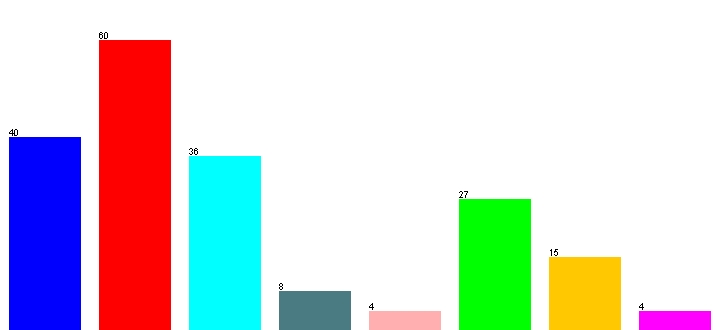
\includegraphics[width=0.75\textwidth]{fig/religion-religion.jpg}%
  \caption{%
    L'istogramma rappresenta i valori assunti dall'attributo utilizzato come classe:
    la colonna blu rappresenta la religione cattolica,
    quella rossa le religioni cristiane non cattoliche, quella azzurra il musulmanesimo,
    quella grigia la fede buddista, quella rosa la religione indù, quella verde la religione
    definita etnica, quella gialla il marxismo, ed infine la colonna viola rappresenta le altre religioni.
  }%
  \label{fig:classes}
\end{figure}

Molto interessante l'attributo \textbf{Continente}, in quanto la distribuzione delle istanze delle classi risulta particolare:
si nota, infatti, dalla~\Cref{fig:landmass} come il continente 4 (ovvero l'\emph{Africa}) contenga quasi tutte le istanze della religione cosiddetta etnica;
o ancora, si può vedere come la religione musulmana risulta presente quasi esclusivamente nei continenti 4 e 5 (ovvero \emph{Africa} e \emph{Asia});
altra informazione interessante riguarda la fede marxista, presente quasi esclusivamente in \emph{Europa} e \emph{Asia} (colonne 3 e 5), con una piccola presenza in \emph{Nord America} (colonna 1).

\begin{figure}[H]
  \centering
  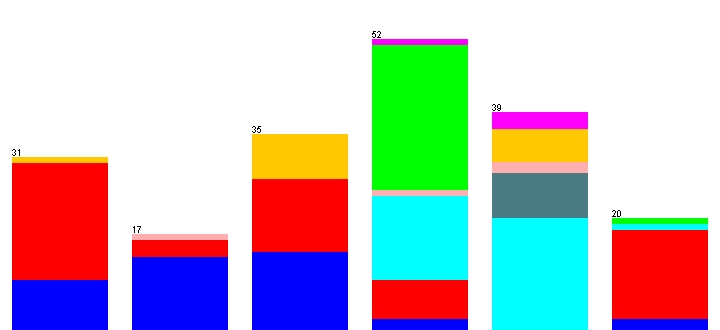
\includegraphics[width=0.75\textwidth]{fig/religion-landmass.jpg}%
  \caption{%
    L'istogramma rappresenta i valori assunti dall'attributo \textbf{Continente}
    all'interno del dataset: le colonne, nell'ordine rappresentano i 6 continenti, rispettivamente,
    Nord America, Sud America, Europa, Africa, Asia ed Oceania.
    }%
  \label{fig:landmass}
\end{figure}

L'attributo \textbf{Zona}, risulta ben distribuito con distribuzioni interessanti delle istanze delle classi.
Nel Sud-OVest (terza colonna), ad esempio, sono presenti poche nazioni, ma tutte con religione Cristiana e Cattolica;
interessante anche la distribuzione delle istanze con religione musulmana: quasi solo nel Nord-Est;
quest'ultima zona comprende quasi esclusivamente le nazioni con fede marxista (probabilmente in quanto Europa ed Asia sono continenti che occupano la stragrande maggioranza del quadrante ad Est del meridiano di Greenwich e a Nord dell'Equatore).

\begin{figure}[H]
  \centering
  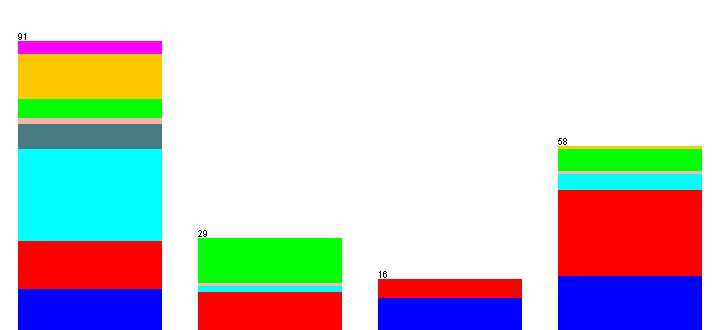
\includegraphics[width=0.75\textwidth]{fig/religion-zone.jpg}%
  \caption{%
    L'istogramma rappresenta i valori assunti dall'attributo \textbf{Zona}
    all'interno del dataset: le colonne, nell'ordine rappresentano i 4 quadranti del mondo, rispettivamente,
    Nord-Est, Sud-Est, Sud-Ovest, Nord-Ovest.
    }%
  \label{fig:zone}
\end{figure}

L'attributo \textbf{Lingua} appare molto interessante, in quanto le istanze della classe sono distribuite in maniera particolare.
Salta all'occhio immediatamente che tutte le 4 nazioni di lingua slava (colonna 5) hanno come fede la religione marxista;
ancora più interessante è la colonna riguardante i paesi di lingua araba (colonna 8): 19 istanze, tutte con religione musulmana;
le 21 istanze di lingua spagnola (colonna 2) sono quasi in totalità di religione cattolica.

\begin{figure}[H]
  \centering
  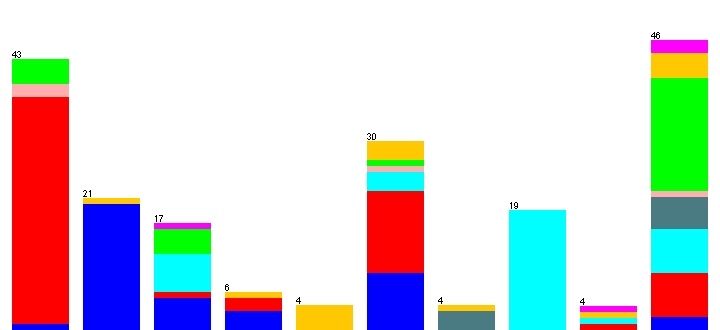
\includegraphics[width=0.75\textwidth]{fig/religion-language.jpg}%
  \caption{%
    L'istogramma rappresenta i valori assunti dall'attributo \textbf{Lingua}
    all'interno del dataset: le colonne, nell'ordine rappresentano le dieci lingue codificate dal dataset, rispettivamente,
    inglese, spagnolo, francese, tedesco, slavo, altre lingue indo-europee, cinese, arabo, giapponese/turco/finlandese/magiaro, altre lingue.
    }%
  \label{fig:language}
\end{figure}

L'attributo rappresentante il numero di \textbf{Colori} nella bandiera nazionale appare distribuito in maniera abbastanza intuitiva.
Le nazioni con bandiere contenenti dai due ai quattro colori sono la stragrande maggioranza, con dei picchi al ribasso di una nazione per entrambi gli estremi: un colore e otto colori.
La distribuzione delle istanze della classe, in questo caso, non risulta ricca di informazioni di primo impatto: unica nota di rilievo consiste nelle nazioni con elevato numero di colori nella bandiera;
queste ultime infatti (ultime quattro colonne, quindi con numero di colori da cinque a otto) sono per grande maggioranza nazioni cristiane non cattoliche.

\begin{figure}[H]
  \centering
  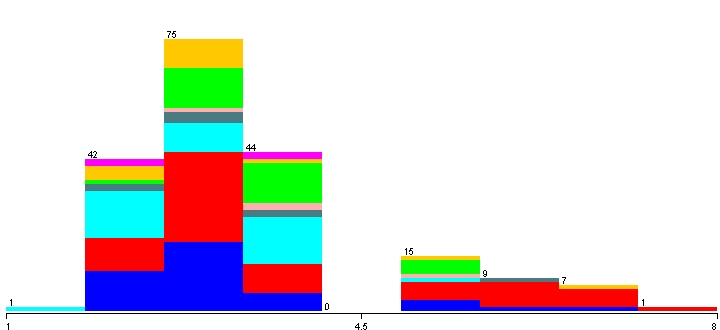
\includegraphics[width=0.75\textwidth]{fig/religion-colours.jpg}%
  \caption{%
    L'istogramma rappresenta i valori assunti dall'attributo \textbf{Colori}
    all'interno del dataset: le colonne, rappresentano il quantitativo di colori presenti nella bandiera di ogni nazione, andando da uno a otto.
    }%
  \label{fig:colours}
\end{figure}

Come si può vedere dalla~\Cref{fig:mainhue}, l'attributo \textbf{Tonalità principale} (in relazione ai colori della bandiera) ha una distribuzione sbilanciata sui primi cinque colori,
ovvero verde, rosso, blu, giallo e bianco. In particolare, la stragrande maggioranza delle nazioni di fede musulmana hanno come tonalità principale il verde o il rosso; altra cosa interessante riguarda la fede marxista:
la maggioranza delle nazioni con questa reigione hanno come tonalità principale della bandiera il rosso.

\begin{figure}[H]
  \centering
  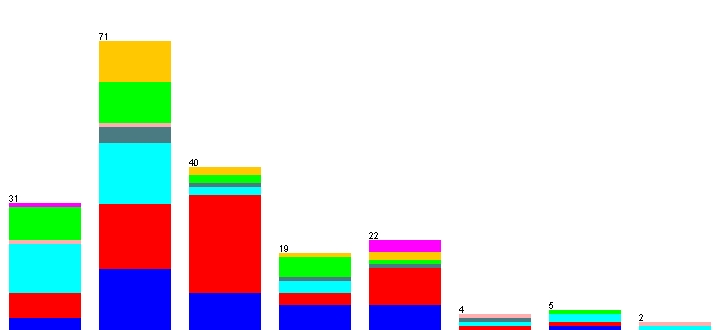
\includegraphics[width=0.75\textwidth]{fig/religion-mainhue.jpg}%
  \caption{%
    L'istogramma rappresenta i valori assunti dall'attributo \textbf{Tonalità principale}
    all'interno del dataset: le colonne, rappresentano, nell'ordine, le tonalità principali assunte dalla bandiera nazionale, rispettivamente
    verde, rosso, blu, oro (o giallo), bianco, arancio, nero e marrone.
    }%
  \label{fig:mainhue}
\end{figure}

La~\Cref{fig:saltires} esprime la distribuzione dell'attributo \textbf{Saltires} (che indica la presenza di croci diagonali nella bandiera).
Questo attributo binario ha uno sbilanciamento verso il valore 0 (ovvero assenza di croci diagonali), ma si può notare come quasi tutte le 18 nazioni con
una croce diagonale nella bandiera sono di religione cristiana non cattolica.

\begin{figure}[H]
  \centering
  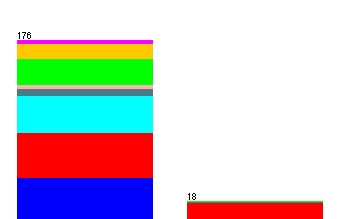
\includegraphics[width=0.75\textwidth]{fig/religion-saltires.jpg}%
  \caption{%
    L'istogramma rappresenta i valori assunti dall'attributo \textbf{Saltires}
    all'interno del dataset: attributo binario, che esprime assenza (prima colonna) o presenza (seconda colonna) di croci diagonali nella bandiera della nazione.
    }%
  \label{fig:saltires}
\end{figure}

La~\Cref{fig:crescent} esprime la distribuzione dell'attributo \textbf{Crescent} (che indica la presenza di figure rappresentanti una luna crescente nella bandiera).
Questo attributo binario ha uno sbilanciamento verso il valore 0 (ovvero assenza di lune crescenti), ma si può notare come quasi tutte le 11 nazioni con
una luna crescente nella bandiera sono di religione musulmana.

\begin{figure}[H]
  \centering
  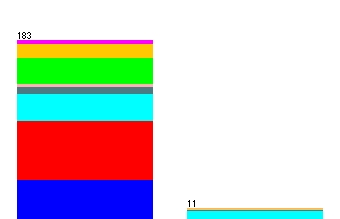
\includegraphics[width=0.75\textwidth]{fig/religion-crescent.jpg}%
  \caption{%
    L'istogramma rappresenta i valori assunti dall'attributo \textbf{Crescent}
    all'interno del dataset: attributo binario, che esprime assenza (prima colonna) o presenza (seconda colonna) di lune crescenti nella bandiera della nazione.
    }%
  \label{fig:crescent}
\end{figure}

La~\Cref{fig:topleft} esprime la distribuzione dell'attributo \textbf{Topleft} (che indica la tonalità di colore presente nell'angolo in alto a sinistra della bandiera).
La distribuzione delle istanze di questo attributo è sbilanciata per quattro colori (rosso, verde, blu e bianco) corrispondenti alle colonne da due a cinque comprese; gli altri colori contano solo ventidue istanze in totale.

\begin{figure}[H]
  \centering
  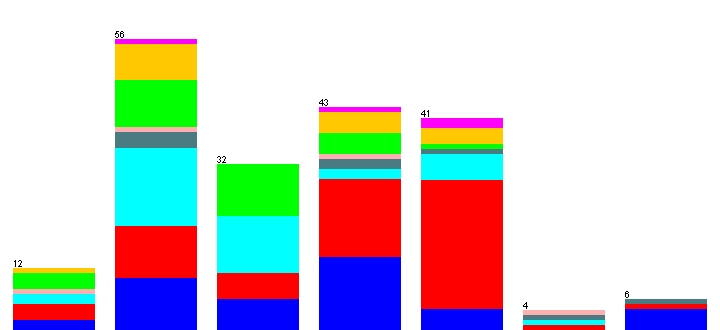
\includegraphics[width=0.75\textwidth]{fig/religion-topleft.jpg}%
  \caption{%
    L'istogramma rappresenta i valori assunti dall'attributo \textbf{Topleft}
    all'interno del dataset: attributo nominale, che indica la tonalità di colore presente nell'angolo in alto a sinistra della bandiera della nazione;
    i colori sono, nell'ordine raffigurato, nero, rosso, verde, blu, bianco, arancio e oro (o giallo).
    }%
  \label{fig:topleft}
\end{figure}

La~\Cref{fig:botright} esprime la distribuzione dell'attributo \textbf{Botright} (che indica la tonalità di colore presente nell'angolo in basso a destra della bandiera).
La distribuzione delle istanze di questo attributo, come per l'attributo precedente, è sbilanciata per quattro colori (rosso, verde, blu e bianco, anche se con meno rilevanza in quest'ultimo) corrispondenti alle colonne da due a cinque comprese; gli altri colori contano solo ventidue istanze in totale.

\begin{figure}[H]
  \centering
  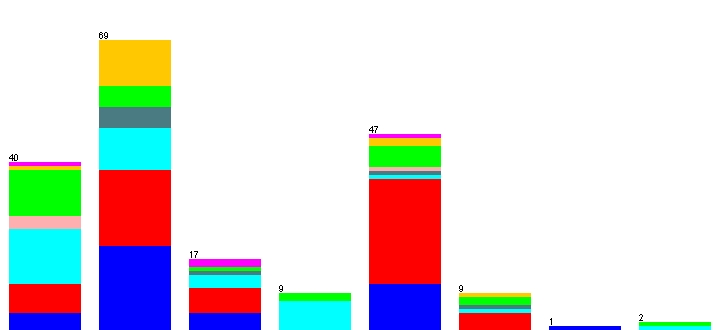
\includegraphics[width=0.75\textwidth]{fig/religion-botright.jpg}%
  \caption{%
    L'istogramma rappresenta i valori assunti dall'attributo \textbf{Botright}
    all'interno del dataset: attributo nominale, che indica la tonalità di colore presente nell'angolo in basso a destra della bandiera della nazione;
    i colori sono, nell'ordine raffigurato, verde, rosso, bianco, nero, blu, oro (o giallo), arancio e marrone.
    }%
  \label{fig:botright}
\end{figure}

\subsection{Misure di performance dei classificatori}

Prima di partire con le analisi, occorre stabilire i criteri di misura delle performance dei vari classificatori:
a tale scopo si è considerato in primo luogo la \emph{Confusion Matrix} prodotta da ogni modello, oltre ai valori di \emph{precision} e \emph{recall} per le classi in gioco, attribuendo un maggiore peso ai valori relativi alle classi con meno istanze e infine del valore della \emph{ROC}\@.

Come modalità di test, si è scelto di applicare \emph{k-Fold Cross-Validation} piuttosto che lo splitting statico dei dati in training set e test set, poiché pensato appositamente per dataset di piccole dimensioni come quello preso in esame.


\subsection{Decision Tree}\label{subsec:tree}

Il primo approccio di classificazione intrapreso è stato il \textbf{Decision Tree}.
In particolare, si è scelto di usare \texttt{J48}, implementazione dell'algoritmo \emph{C4.5} presente all'interno del software \emph{Weka};
esso realizza un albero binario a cui possono essere applicate tecniche di \emph{post pruning}
per ridurre le dimensioni dell'albero e l'errore commesso dal classificatore.

\begin{figure}[H]
  \centering
  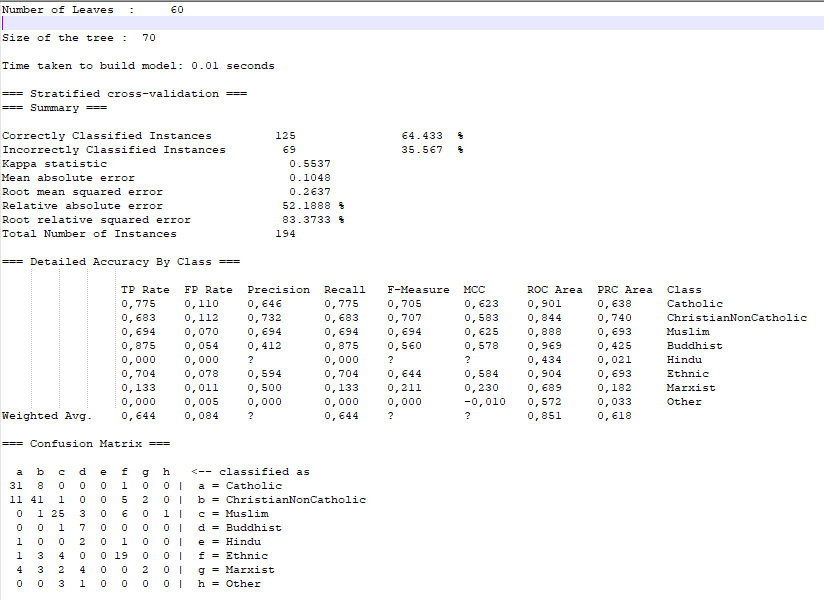
\includegraphics[width=0.75\textwidth]{fig/DecisionTree1.PNG}%
  \caption{Output di \texttt{J48} eseguito tramite Weka}%
  \label{fig:j48}
\end{figure}

Si è innanzitutto tentato di generare un modello applicando i parametri standard impostati da Weka, ottenendo così i risultati riportati in~\Cref{fig:j48}.
Com'è possibile notare, il classificatore costruisce un modello non particolarmente valido, in particolare per due delle classi con meno istanze:
infatti, i valori di \emph{accuracy}, \emph{precision} e \emph{recall} hanno valori pari a \(0\) per le religioni \textbf{Indù} e \textbf{Altre}, mentre hanno valori vicino a \(0\) per la religione \textbf{Marxista}.
Anche il valore di \emph{ROC}, indicatore principale della bontà di un modello di classificazione, risulta in linea con queste sensazioni, infatti è molto basso (vicino o sotto a 0,5) per le classi sopra citate.

La struttura dell'albero costruito, risulta che le classi per cui i valori sono pari a \(0\) non vengono assegnate ad alcuna foglia, causando
così la situazione sopra descritta.

Ovviamente questo modello non risultava di una qualità soddisfacente per queste classi, probabilmente a causa del post pruning,
il quale, in presenza di un tale sbilanciamento nella frequenza delle classi meno popolate, tende a ridurre il numero di foglie dell'albero di classificazione.
Per porre rimedio a questa cosa si è provato ad aumentare e diminuire il parametro \texttt{confidenceFactor}, responsabile di accentuare o smussare le operazioni di pruning;
anche però variando questo parametro i risultati ottenuti non sono stati particolarmente differenti.

Si è pensato, dunque, di disattivare il pruning (tramite il flag \texttt{unpruned}): la situazione è leggermente migliorata localmente per la classe \emph{Other},
a scapito di due istanze classificate non correttamente nel complesso, come è possibile vedere in~\Cref{fig:j48-unpruned}.


\begin{figure}[H]
  \centering
  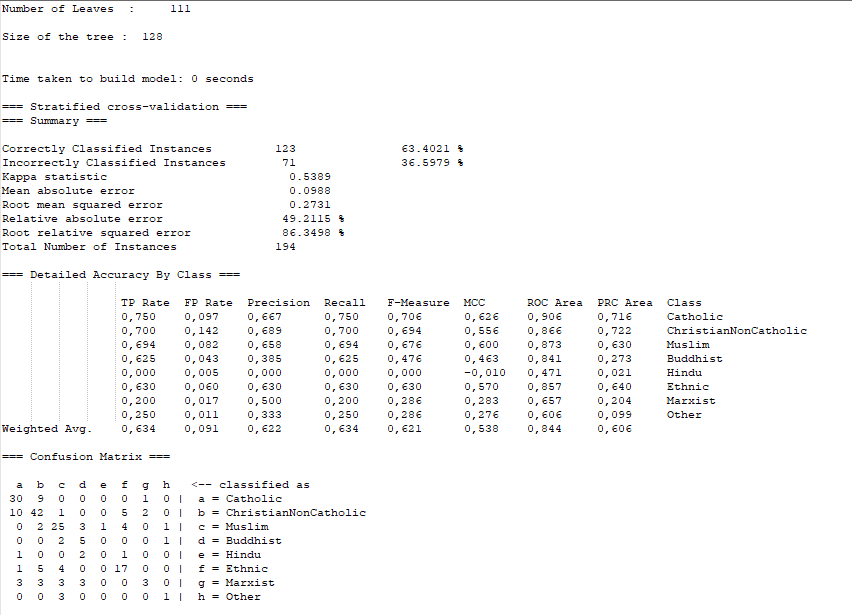
\includegraphics[width=0.75\textwidth]{fig/DecisionTree2.PNG}%
  \caption{Albero di classificazione e output ottenuti con \texttt{J48} \emph{unpruned}}%
  \label{fig:j48}
\end{figure}

Il risultato del classificatore non risulta migliore rispetto alla sua versione \emph{pruned}, tuttavia consente di classificare meglio quelle classi con poche istanze,
a scapito, appunto, delle classi più popolate, rendendo complessivamente meno performante la classificazione (anche se di poco).

Sperimentando ulteriormente con la versione \emph{unpruned} di \texttt{J48},
abbassando il numero minimo di elementi per foglia a \(1\) il valore di \emph{recall} per la classe \texttt{Altre} e di \emph{True Positive} si alzava,
ma il valore di \emph{ROC} e \emph{precision} si abbassavano, anche se di molto poco; ma i corrispondenti valori per le altre classi peggioravano.

Cercando di alzare il numero minimo di elementi per foglia, continuavano a ottenersi risultati ancora peggiori.

Si può dunque concludere che il classificatore \texttt{J48} non garantisce risultati ottimali su questo dataset, soprattutto a causa del grande sbilanciamento tra le distribuzioni delle classi.

\subsection{Classificatori Bayesiani: \emph{Naïve Bayes}}\label{subsec:bayes}

Per tentare un approccio differente, ho provato a costruire un modello basato sui classificatori bayesiani,
approccio che ignora le relazioni tra gli attributi in favore della frequenza di certi valori rispetto alle classi in gioco.

Il classificatore specifico scelto per il dataset è stato \emph{Naïve Bayes} nella sua implementazione fornita da Weka (chiamata appunto \texttt{NaiveBayes});
costruendo il modello utilizzando i parametri standard impostati dalla workbench, sono stati ottenuti i risultati mostrati in~\Cref{fig:bayes}.


\begin{figure}[H]
  \centering
  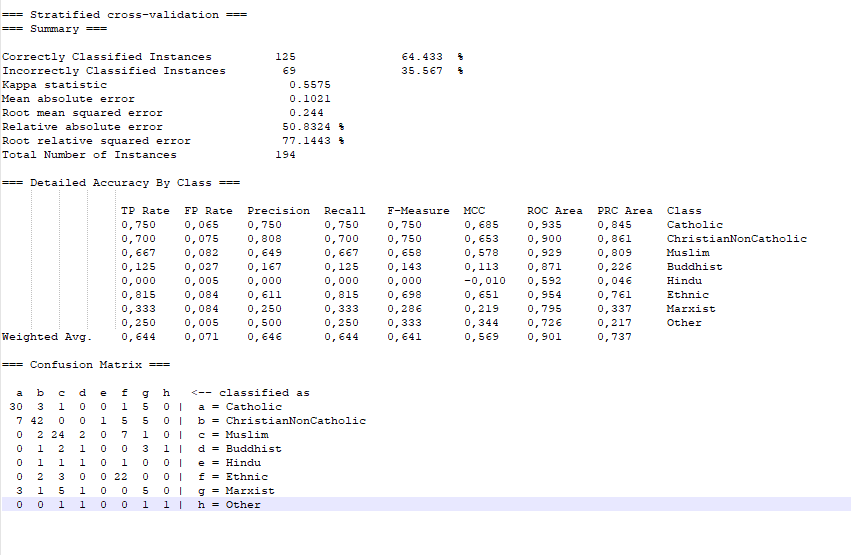
\includegraphics[width=0.75\textwidth]{fig/bayes.PNG}%
  \caption{Output di \texttt{NaiveBayes} eseguito tramite Weka}%
  \label{fig:bayes}
\end{figure}

Analizzando i risultati di questo classificatore, si possono fare alcune considerazioni:
partendo dall'osservazione della \emph{confusion matrix} è possibile vedere come tutte le classi con il maggior numero di istanze (``\texttt{Cattolica}'', ``\texttt{Cristiana non cattolica}'', ``\texttt{Musulmana}'', ``\texttt{Etnica}'')
vengono classificate con errori relativamente bassi, mentre la classificazione per le altre risulta molto meno affidabile; nel complesso, la classificazione non mostra risultati troppo differenti da quella eseguita utilizzando il modello ad Albero Decisionale.

Solo la classe ``\texttt{Indù}'' mostra valori di \emph{precision} e \emph{recall} pari a \(0\), ma anche le altre classi con poche istanze presentano valori di questo tipo molto bassi, pur non arrivando a \(0\).

Infine, osservando \emph{ROC} si ha la conferma definitiva che il modello costruito sia poco performante per questo tipo di classi.

Le ragioni dietro alla poca efficienza del modello bayesiano per questo problema possono essere ricondotte alla mancanza dei valori di distribuzione delle probabilità reali per le classi e alla potenziale mancanza di indipendenza statistica tra attributi.
Questi fattori, combinati allo sbilanciamento dei dati nel dataset, da cui vengono estratte le distribuzioni di probabilità necessarie al classificatore in mancanza di quelle reali, rendono inefficace il modello bayesiano su questo dataset.

\subsection{Classificatori Lazy: \emph{k-NN}}\label{subsec:ibk}

Altra famiglia utilizzata è stata quella dei \emph{classificatori Instance-based} o \emph{Lazy}.
La particolarità di queste tecniche è la totale assenza di modello, sostituito da procedure di natura induttiva.

Tra tutti i classificatori disponibili in questa famiglia, si è scelto di utilizzare \texttt{IBk}, implementazione in Weka dell'algoritmo \emph{k-NN};
per questo classificatore è possibile impostare diversi parametri, come il numero di vicini da considerare e la metrica da utilizzare nel calcolo della distanza.

Applicando i parametri default di Weka, ovvero con parametro \texttt{KNN=1} e \emph{distanza euclidea}, si ottengono i risultati riportati in~\Cref{fig:ibk:1}.

\begin{figure}[H]
  \centering
  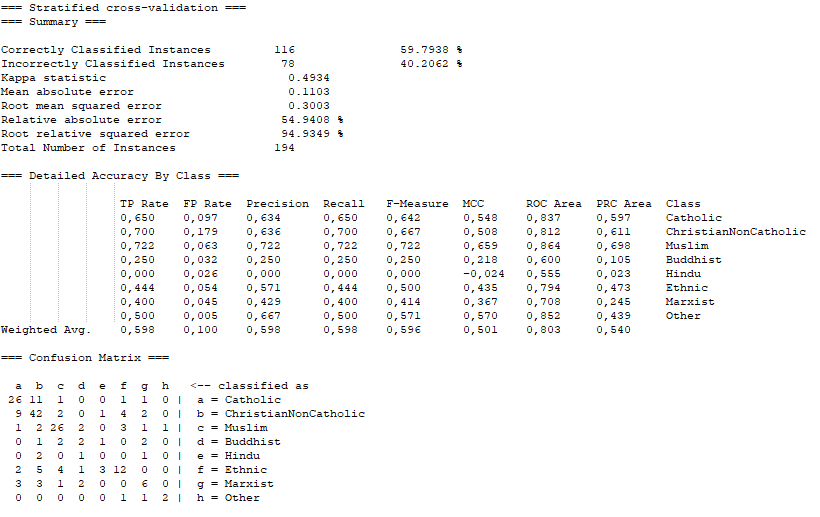
\includegraphics[width=0.75\textwidth]{fig/kNN1.PNG}%
  \caption{Output di \texttt{IBk} eseguito tramite Weka}%
  \label{fig:ibk:1}
\end{figure}

I risultati ottenuti da questo modello risultano particolarmente cattivi per le classi con maggior numero di istanze, notevolmente peggiori di quelli ottenuti utilizzando i modelli precedenti.
Si riscontrano, in questo caso, valori di \emph{precision} e \emph{recall} pari a \(0\) solo per la classe \texttt{Indù}.
Si è ritenuto dunque di poter migliorare il modello utilizzando valori differenti per i parametri sopra descritti.

Mantenendo la \emph{distanza euclidea} come metrica, si è provato a variare il valore di K tra i numeri dispari compresi tra \(3\) e \(11\);
questa modifica ha portato migliorie (seppur molto leggere), per le classi con molte istanze, solamente con \texttt{KNN=3} e \texttt{KNN=5}.
Ma il risultato non è stato ritenuto comunque accettabile considerando i valori ottenuti in \emph{precision} e \emph{recall} e la percentuale di istanze correttamente e incorrettamente classificate.

\begin{figure}[H]
  \centering
  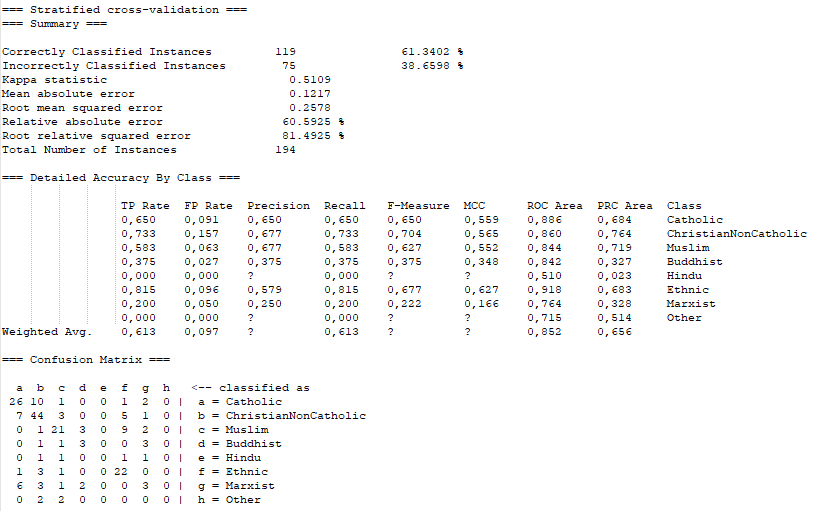
\includegraphics[width=0.75\textwidth]{fig/kNN3.PNG}%
  \caption{Output di \texttt{IBk} con \texttt{KNN=3}}%
  \label{fig:ibk:9}
\end{figure}

Si è pensato, infine, di \textbf{pesare} le distanze calcolate dall'algoritmo, in quanto con un numero così elevato di classi rispetto al numero relativamente esiguo di record del dataset, avrebbe potuto aiutare un algoritmo basato sulla distanza come il \texttt{kNN}.
Settando propriamente il parametro \texttt{distanceWeighting} all'interno dell'interfaccia \emph{Weka}, le distanze sono state pesate come ``\texttt{1--distance}''.

I risultati così ottenuti risultano più soddisfacenti per i valori \emph{ROC}, mantenendo inalterato il valore \texttt{KNN=3}.

\begin{figure}[H]
  \centering
  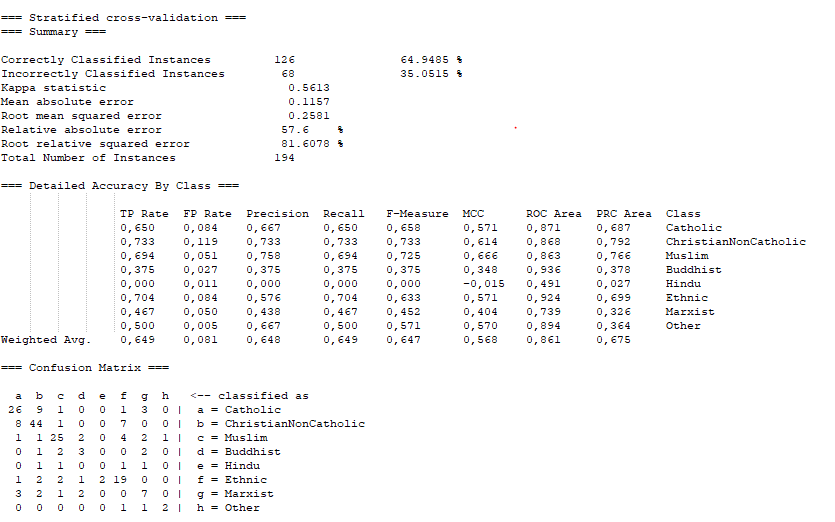
\includegraphics[width=0.75\textwidth]{fig/kNNWeighted.PNG}%
  \caption{Output di \texttt{IBk} con \texttt{KNN=3} e la distanza pesata come \texttt{1--distance}}%
  \label{fig:ibk:9}
\end{figure}

\subsection{Multi-Classificatori}

I classificatori precedentemente descritti non hanno portato a un modello particolarmente efficace;
si è dunque deciso di provare ad utilizzare modelli a multi-classificatori.
Tali classificatori sono infatti noti per essere particolarmente efficaci per problemi in cui classificatori singoli faticano a raggiungere performance accettabili.

Tra le varie possibilità messe a disposizione da Weka, si è scelto di utilizzare due diversi algoritmi:
\emph{Cost-Sensitive Classifier}, modello che permette di gestire dataset sbilanciati in partenza per distribuzioni delle classi e \emph{Adaboost}, classificatore appartenente alla famiglia delle tecniche di \emph{Boosting}.

\subsubsection{Approccio Cost-Sensitive}

I multi-classificatori \emph{cost-sensitive} sono generalmente efficaci nel gestire dataset non bilanciati, come in questo caso;
essi infatti consentono di attribuire un peso alle istanze sbagliate delle varie classi in gioco, eseguendo così una procedura di \emph{model tuning}.

L'implementazione disponibile in Weka, chiamata \texttt{CostSensitiveClassifier},
permette di selezionare un \emph{classificatore} (i cui parametri possono essere settati a piacere) su cui costruire un modello
e una \emph{matrice di costo} di dimensione \(N×N\) (dove \(N\) è il numero di classi in gioco) con la quale è possibile assegnare una differente penalità alle istanze classificate per ogni classe.

Il primo classificatore provato è stato \texttt{J48}, specificando vari valori nella matrice di costo (accrescendo sempre più la penalità dovuta all'errata classificazione delle classi con meno istanze quali ``\texttt{Indù}'' e ``\texttt{Altre}''):
al crescere del peso, effettivamente queste classi risultavano favorite, ma questo andava a scapito della bontà complessiva della classificazione; infatti, le classi con maggior numero di istanze quali ``\texttt{Cattolica}'', ``\texttt{Cristiana non cattolica}'' o ``\texttt{Musulmaba}'', avevano rendimento sempre peggiore.

Si è cercato dunque di bilanciare le penalità anche per queste classi più grandi, ottenendo, tuttavia, l'effetto contrario: le classi con poche istanze tornavano ad essere più deboli, e quindi mal classificate dal modello.
Purtroppo, avendo un così elevato numero di classi, riuscire a bilanciare le penalità della \emph{cost matrix} risulta particolarmente complesso.

Il valore che sembra garantire il migliore equilibrio, tra quelli trovati, è quello riportato in~\Cref{fig:cost:j48}.

\begin{figure}[H]
  \centering
  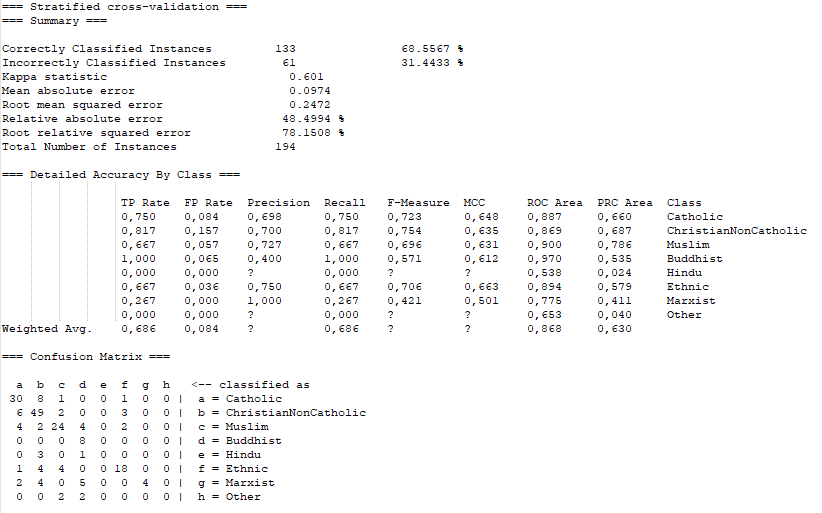
\includegraphics[width=0.75\textwidth]{fig/MultiJ48.PNG}%
  \caption{Output di \texttt{CostSensitiveClassifier} con \texttt{J48}}%
  \label{fig:cost:j48}
\end{figure}

Utilizzando invece come classificatore base il \emph{Naïve Bayes}, i risultati migliorano leggermente rispetto al solo classificatore bayesiano, tuttavia le performance rimangono inferiori rispetto al modello costruito con \emph{J48} (anche se i valori di \emph{ROC} anche per le classi con poche istanze risultano migliori, a scapito di \emph{precision} e \emph{recall});
probabilmente nonostante l'approccio \emph{cost-based} migliori l'efficacia del modello \texttt{NaiveBayes}, le problematiche espresse nella~\Cref{subsec:bayes} sono talmente importanti da non rendere il classificatore valido nemmeno così utilizzato.

\begin{figure}[H]
  \centering
  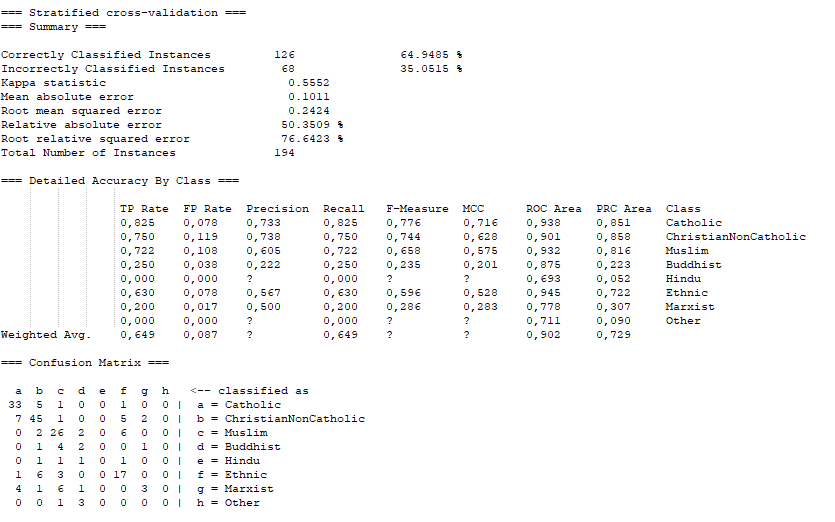
\includegraphics[width=0.75\textwidth]{fig/MultiBayes.PNG}%
  \caption{Output di \texttt{CostSensitiveClassifier} con \emph{Naïve Bayes}}%
  \label{fig:cost:j48}
\end{figure}

Infine è stato utilizzato come classificatore base \texttt{IBk}, che aveva garantito i risultati migliori finora.
Applicando i modelli descritti nella~\Cref{subsec:ibk}, i risultati ottenuti non sono stati altrettanto validi:
il miglior risultato in assoluto (\Cref{fig:cost:ibk5}) è stato ottenuto utilizzando \texttt{KNN=5}, \emph{distanza euclidea} e penalità per i record mal classificati simili a quelli utilizzati per l'algoritmo \emph{J48}.

\begin{figure}[H]
  \centering
  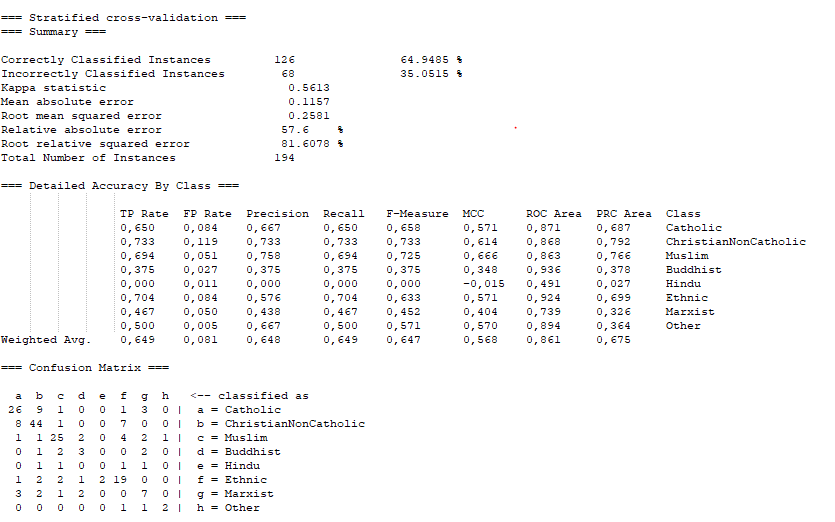
\includegraphics[width=0.75\textwidth]{fig/kNNWeighted.PNG}%
  \caption{Output di \texttt{CostSensitiveClassifier} con \texttt{IBk} con \texttt{KNN=5}}%
  \label{fig:cost:ibk5}
\end{figure}

\subsubsection{Approccio Boosting}

L'ultimo approccio tentato è stato il \emph{boosting}, processo che si basa sulla costruzione di più classificatori attribuendo ogni volta un peso maggiore agli elementi mal classificati al passo precedente.

Come per i \emph{classificatori cost-based}, anche qui è possibile specificare un modello di base per costruire la classificazione:
in modo analogo sono stati testati tutti i tre classificatori base impiegati ai passi precedenti nelle \Cref{subsec:tree,subsec:bayes,subsec:ibk},
ottenendo i risultati migliori, anche se comunque complessivamente peggiori rispetto all'approccio con i \emph{classificatori cost-based}, con \texttt{NaiveBayes}.
In \Cref{fig:adaboost:bayes} sono riportati i risultati ottenuti con \texttt{NaiveBayes} come classificatore base, e un numero di iterazioni pari a \(10\).

\begin{figure}[H]
  \centering
  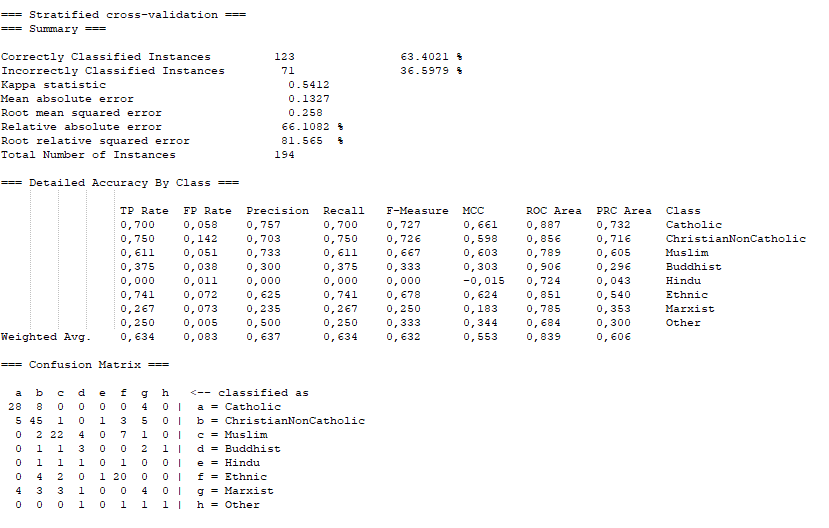
\includegraphics[width=0.75\textwidth]{fig/AdaboostBayes.PNG}%
  \caption{Output di \texttt{AdaboostM1} con \texttt{NaiveBayes} e \(10\) iterazioni}%
  \label{fig:adaboost:bayes}
\end{figure}

I risultati per questo modello non sono particolarmente buoni: per la classe ``\texttt{Altre (religioni ndr.)}'' risultano migliori i valori di \emph{precision} e \emph{recall} (anche se comunque ancora bassi),
mentre per le classe con un maggior numero di istanze, questi valori risultano peggiori rispetto a quelli ottenuti con i \emph{classificatori cost-based}.

\newpage

\section{Conclusioni}

\todo[shadow]{Until here ---------------}

Lo studio di questo dataset è stato sicuramente molto interessante, per quanto fosse complicato da analizzare;
partendo da risultati non ottimali, è stato necessario valutare bene la struttura stessa del dataset e il funzionamento dei classificatori
interpretare i risultati di ciascuna prova.

In primo luogo, si può affermare che i modelli basati sui \emph{classificatori Lazy} producono i risultati più solidi, sebbene ancora lontani da potersi definire efficienti.
La ragione di tale solidità può essere attribuita alla maggiore resistenza del classificatore a uno sbilanciamento della frequenza delle classi nel dataset rispetto agli altri modelli impiegati.

In secondo luogo, l'impiego di multi-classificatori, sia \emph{boosting} che \emph{cost-sensitive},
ha permesso di migliorare ulteriormente le misure di bontà e la classificazione delle istanze della classe ``\texttt{O}'', che sarebbe poi quella più rilevante.
Tra i due, si ritiene che non si abbia un modello migliore dell'altro, bensì che tutto dipenda dal contesto in cui vengono applicati:
se ad esempio l'obiettivo è identificare il maggior numero di potenziali pazienti con problemi di sterilità, allora conviene utilizzare il modello \emph{cost-sensitive};
al contrario se l'interesse primario è avere un sistema che sia il più vicino possibile alla realtà modellata dai dati, allora il modello basato su \emph{Adaboost} potrebbe essere la scelta migliore.

\end{document}
